\section{Realisatie}

\subsection{De ISFET}

Aan de ingang van de signaalverwerking van de pH waarde, zit de sensor die deze pH waarde uitleest, zoals te zien in \cref{fig:pHInSchema}. Deze sensor meet de pH waarde van de te meten oplossing. De sensor die wordt gebruikt is een ISFET halfgeleider.
\begin{figure}[!htbp]
    \centering
    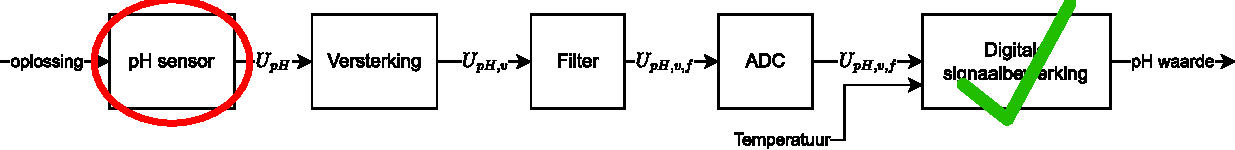
\includegraphics[width=0.95\textwidth]{signaalverwerking_pH.pdf}
    \caption{Het onderdeel van \cref{fig:analogeBewerkingsFunctie} waar dit hoofdstuk over gaat.}
    \label{fig:pHInSchema}
\end{figure}

De pH sensor heeft als ingang een oplossing met een pH waarde van pH 2 tot pH 10. De uitgang is een spanning tussen de \qty{1.8}{\volt} en \qty{2.2}{\volt} \cite{isfet}, die lineair afhankelijk is van de pH waarde. Dit is te zien in \cref{fig:uitleesBlok}.

\begin{figure}[!htbp]
    \centering
    \def\svgwidth{0.4\textwidth}
    \input{img/uitleesBlok.pdf_tex}
    \caption{De in- en uitgangen van de uitleesschakeling.}
    \label{fig:uitleesBlok}
\end{figure}


\subsubsection{De drempelspanning van de ISFET uitlezen} \label{sec:ISFETLees}
Wanneer de ISFET in aanraking komt met een oplossing, verandert de gate-source drempelspanning op basis van de pH waarde van deze oplossing \cite{bergveld2003thirtyYearsISFET,bergveld1985impactOfMosfetBasedSensors}. Om deze uit te lezen kan een regelsysteem gebruikt worden om de drain-source spanning en stroom van de ISFET mee in te stellen.

Er zijn meerdere mogelijke implementaties mogelijk voor dit regelsysteem. Twee hiervan zijn afgebeeld in \cref{fig:measureCircuits}.
Elk van deze schakelingen gebruikt een nullor om de drain-source spanning van de ISFET gelijk te houden. Ook gebruikt elk van deze schakelingen een referentiespanning. De implementatie van deze referentiespanning wordt verder besproken in \cref{sec:referenceVoltage}.

De drain-source spanning $U_{ds}$ en drain-source stroom $I_{ds}$ zijn van te voren gedefinieerd. Deze zijn te vinden in de datasheet van de ISFET \cite{isfet}. Uit deze twee waardes kunnen de referentiespanningen en weerstandswaardes van de schakelingen gevonden worden.
Voor de schakeling in \cref{fig:measureCurrent} is de spanningsreferentie te vinden door middel van \cref{eq:URefSource}.
\begin{equation}\label{eq:URefSource}
    U_{ref,s} = U_{dd} - U_{ds}
    \tagaddtext{[\si{\volt}]}
\end{equation}
Voor \cref{fig:measureResistor} is de referentiespanning gelijk aan de drain-source spanning, te zien in \cref{eq:URefDrain}.
\begin{equation}\label{eq:URefDrain}
    U_{ref,d} = U_{ds}
    \tagaddtext{[\si{\volt}]}
\end{equation}
Voor de waarde van de weerstand in \cref{fig:measureResistor} kan \cref{eq:measureResistorVal} gebruikt worden.
\begin{equation}\label{eq:measureResistorVal}
    R = \frac{U_{dd} - U_{ds}}{I_{ds}}
    \tagaddtext{[\si{\ohm}]}
\end{equation}


\begin{figure}[!htbp]
    \centering
    \begin{subfigure}[b]{0.45\textwidth}
        \centering
        \def\svgwidth{\textwidth}
        \input{img/ISFETCircuitBest.pdf_tex}
        \caption{Met een weerstand aan de drain.}
        \label{fig:measureResistor}
    \end{subfigure}
    \hfill
    \begin{subfigure}[b]{0.45\textwidth}
        \centering
        \def\svgwidth{\textwidth}
        \input{img/ISFETCircuit.pdf_tex}
        \caption{Met een stroombron aan de source.}
        \label{fig:measureCurrent}
    \end{subfigure}
    \caption{De uitleesschakelingen voor de ISFET.}
    \label{fig:measureCircuits}
\end{figure}

Beide schakelingen hebben voor- en nadelen.
Bij de schakeling in \cref{fig:measureResistor} zit de source van de ISFET direct verbonden met de ground. Dit heeft als voordeel dat de uitgang van de nullor gelijk is aan de gate-source spanning. Hierdoor hoeft de nullor lagere spanningen te genereren om de gate-source spanning van de ISFET naar de goede waarde te krijgen. De spanning die de nullor moet genereren in het geval van een drain weerstand is te vinden door middel van \cref{eq:nullorVoltageDrain}. In het geval van een stroombron aan de source is dat \cref{eq:nullorVoltageSource}.

\begin{equation}\label{eq:nullorVoltageDrain}
    U_{nullor,d} = U_{gs}
    \tagaddtext{[\si{\volt}]}
\end{equation}
\begin{equation}\label{eq:nullorVoltageSource}
    U_{nullor,s} = U_{gs} + U_{ref,s}
    \tagaddtext{[\si{\volt}]}
\end{equation}

De schakeling met een stroombron aan de source heeft de mogelijkheid om betere ruiseigenschappen te hebben. De stroombron kan ook een hogere impedantie hebben dan de weerstand. Het vermogensverbruik van de schakeling in \cref{fig:measureResistor} is echter duidelijk minder, dus is dit de schakeling die gebruikt zal worden.

\subsubsection{Ruis van de ISFET uitleesschakeling}

De meetschakeling heeft een aantal ruisbronnen. De nullor heeft een ingangsstroom- en spanningsruisbron. Daarnaast genereert de weerstand ook thermische ruis. Deze ruisbronnen zijn te zien in \cref{fig:measureNoise}.
\begin{figure}[!htbp]
    \centering
    \def\svgwidth{0.6\textwidth}
    \input{img/ISFETCircuitBestNoise.pdf_tex}
    \caption{De ruisbronnen van de meetschakeling.}
    \label{fig:measureNoise}
\end{figure}


Omdat $U_{ds}$ en $I_{ds}$ van de ISFET niet veranderen, kan de impedantie ervan gezien worden als weerstand, met een waarde van $\frac{U_{ds}}{I_{ds}}$. Hierdoor wordt er een nieuwe ruisbron $i_{n,ds}$ toegevoegd. Met deze weerstand kunnen de bronnen $i_{n,ref}$, $i_{n,R}$ en $i_{n,ds}$ worden getransformeerd naar een spanningsbron $u_{n,in}$ aan de ingang van de nullor.
Vervolgens kan deze, samen met de spanningsruisbronnen $u_{n,ref}$ en $u_{n,n}$ naar de uitgang getransformeerd worden. Dit komt uit op een enkele spanningsruisbron aan de uitgang, zoals te zien is in \cref{fig:measureNoiseMoved}. De spectrale spanningsruis dichtheid van deze ruisbron is te berekenen door middel van \cref{eq:measureNoiseOut}.

\begin{equation}\label{eq:measureNoiseOut}
    S_{u_{{n,out}}} = \left(S_{u_{{n,ref}}} + S_{u_{{n,n}}} + S_{i_{n,in}}\left(Z_{fet} // R\right)^2\right) \cdot H^2(\ph)
    \tagaddtext{[\si{\volt\squared\per\hertz}]}
\end{equation}
\begin{equation}
    S_{i_{{n,in}}} = S_{i_{{n,n}}} + S_{i_{{n,R}}} + S_{i_{{n,ds}}}
    \tagaddtext{[\si{\ampere\squared\per\hertz}]}
    \label{eq:measureNoiseCurrentIn}
\end{equation}


De definities van deze ruisbronnen zijn te vinden in \cref{tab:measureNoiseValues}.

\begin{table}[!htbp]
    \centering
    \begin{tabular}{c|l}
        Ruisbron & Waarde \\
        \hline
        $S_{u_{{n,ref}}}$ & Zie \cref{sec:referenceVoltage} \\
        $S_{u_{{n,n}}}$   & Implementatie nullor \\
        $S_{i_{{n,n}}}$   & Implementatie nullor \\
        $S_{i_{n,in}}$    & \Cref{eq:measureNoiseCurrentIn} \\
        $S_{i_{{n,R}}}$   & $\frac{4kT}{R}$ \\
        $S_{i_{{n,ds}}}$  & $4kT\frac{I_{ds}}{U_{ds}}$ \\
    \end{tabular}
    \caption{Waar de waardes van de ruisbronnen vandaan gehaald kunnen worden.}
    \label{tab:measureNoiseValues}
\end{table}

\begin{figure}[!htbp]
    \centering
    \def\svgwidth{0.6\textwidth}
    \input{img/ISFETCircuitBestNoiseMoved.pdf_tex}
    \caption{De meetschakeling met verschoven ruisbronnen.}
    \label{fig:measureNoiseMoved}
\end{figure}

De overdracht van deze schakeling is gelijk aan de uitgangsspanning gedeeld door de ingangsspanning van de nullor. Door de werking van de schakeling blijft de ingangsspanning altijd gelijk en is de uitgangsspanning lineair afhankelijk van de pH waarde. Hierdoor is de overdracht $H(\ph)$ een functie van de gemeten pH waarde.

Deze overdrachtsfunctie is gedefinieerd in \cref{eq:measureTransfer}, en is een functie van de uitgangsspanning. De uitgangsspanning is een functie van de pH waarde, en is te vinden in \cref{eq:measureOutVoltage}. Hierin is $C_{pH}$ de gevoeligheid van de sensor, die gegeven wordt in $\si{\milli\volt\per\ph}$, en is $U_7$ de uitgangsspanning op pH 7.

\begin{equation}
    H(\ph) = \frac{U_o(\ph)}{U_{ref}}
    \label{eq:measureTransfer}
\end{equation}

\begin{equation}\label{eq:measureOutVoltage}
    U_o(\ph) = C_{pH}\ph + U_7
    \tagaddtext{[\si{\volt}]}
\end{equation}
Door de hoogste uitgangsspanning $U_{o,max}$ te nemen, kan de maximale uitgangsruis berekend worden. Deze is te vinden in \cref{eq:measureNoiseFull}.

\begin{equation}\label{eq:measureNoiseFull}
    S_{u_{{n,out}}} = \left(S_{u_{{n,ref}}} + S_{u_{{n,n}}} + S_{i_{{n,in}}}\left(Z_{fet} // R\right)^2\right) \cdot \left(\frac{U_{o,max}}{U_{ref}}\right)^2
    \tagaddtext{[\si{\volt\squared\per\hertz}]}
\end{equation}

Aangezien er geen frequentieafhankelijkheden voorkomen kan de uitgangsspanningsruis uitgerekend worden door de spectrale ruisdichtheid te vermenigvuldigen met de bandbreedte. Dit wordt gedaan in \cref{eq:measureNoiseVoltage}.
\begin{equation}\label{eq:measureNoiseVoltage}
    u_{n,out} = \sqrt{B \cdot S_{u_{{n,out}}}}
    \tagaddtext{[\si{\volt}]}
\end{equation}

\subsubsection{Vermogen van de ISFET uitleesschakeling}
Het vermogensverbruik van deze schakeling is gedefinieerd in \cref{eq:measurePower}, waar $P_n$ het vermogensverbruik van de nullor implementatie is.
\begin{equation}\label{eq:measurePower}
    P = P_n + U_{dd}I_{ds}
\end{equation}


% \subsubsection{Versterker}
% Aangezien de uitgang van de ISFET een meetbare spanning produceert (\qty{1.8}{\volt} tot \qty{2.2}{\volt} volgens \cite{isfet}) zal er geen versterker nodig zijn om de pH waarde te kunnen meten. Wel zou een level-shifter gebruikt kunnen worden in combinatie met een versterker om zo het volledige bereik van de ADC te gebruiken. Dit voegt echter meer ruis en complexiteit toe aan het systeem, waardoor er in deze iteratie voor is gekozen om dit niet te doen.
%TODO: dit^^
\subsection{Spanningsreferentie}\label{sec:referenceVoltage}

De ISFET uitleesschakeling heeft een spanningsreferentie nodig om te werken.
% TODO: Vertel misschien over andere methoden.
Hiervoor is als implementatie een spanningsdeler gekozen. De schakeling van deze spanningsdeler is te zien in \cref{fig:divider}.
De condensator wordt gebruikt om ruis te verminderen op hogere frequenties, en dient ook als filter voor hoogfrequente storing in de voedingsspanning.

\begin{figure}[!htbp]
    \centering
    \def\svgwidth{0.5\textwidth}
    \subsection{Spanningsreferentie}\label{sec:referenceVoltage}

De ISFET uitleesschakeling heeft een spanningsreferentie nodig om te werken.
% TODO: Vertel misschien over andere methoden.
Hiervoor is als implementatie een spanningsdeler gekozen. De schakeling van deze spanningsdeler is te zien in \cref{fig:divider}.
De condensator wordt gebruikt om ruis te verminderen op hogere frequenties, en dient ook als filter voor hoogfrequente storing in de voedingsspanning.

\begin{figure}[!htbp]
    \centering
    \def\svgwidth{0.5\textwidth}
    \subsection{Spanningsreferentie}\label{sec:referenceVoltage}

De ISFET uitleesschakeling heeft een spanningsreferentie nodig om te werken.
% TODO: Vertel misschien over andere methoden.
Hiervoor is als implementatie een spanningsdeler gekozen. De schakeling van deze spanningsdeler is te zien in \cref{fig:divider}.
De condensator wordt gebruikt om ruis te verminderen op hogere frequenties, en dient ook als filter voor hoogfrequente storing in de voedingsspanning.

\begin{figure}[!htbp]
    \centering
    \def\svgwidth{0.5\textwidth}
    \input{img/divider.pdf_tex}
    \caption{De schakeling van de spanningsdeler die dient als spanningsreferentie.}
    \label{fig:divider}
\end{figure}

De overdracht van deze spanningsdeler is te vinden in \cref{eq:dividerTransfer}.
\begin{equation}\label{eq:dividerTransfer}
    H(s) = \frac{U_{ref}(s)}{U_{dd}(s)} = \frac{R_2}{R_1 + R_2 + R_2Cs}
\end{equation}

\subsubsection{Vermogen}
Het vermogen dat de spanningsdeler dissipeert, kan met \cref{eq:dividerPower} berekend worden.
\begin{equation}\label{eq:dividerPower}
    P(s) = U_{dd}^2(s)\frac{1+R_2Cs}{R_1 + R_2 + R_1R_2Cs}
    \tagaddtext{[\si{\watt}]}
\end{equation}
Met een constante DC ingangsspanning kan dit vereenvoudigd worden naar \cref{eq:dividerPowerSimple}.
\begin{equation}\label{eq:dividerPowerSimple}
    P = \frac{U_{dd}^2}{R_1 + R_2}
    \tagaddtext{[\si{\watt}]}
\end{equation}

\subsubsection{Ruis}
Om de ruis van deze schakeling te berekenen moet een aantal stappen genomen worden. Aangezien de ingangsbron $U_{dd}$ een spanningsbron is, kan deze als kortsluiting genomen worden. Op deze manier kunnen de twee weerstanden parallel genomen worden, en verandert de schakeling in een simpel RC filter. In \cref{fig:dividerNoise} is deze omgebouwde schakeling te zien.

\begin{figure}[!htbp]
    \centering
    \def\svgwidth{0.35\textwidth}
    \input{img/dividerNoise.pdf_tex}
    \caption{De omgebouwde schakeling om ruis mee te berekenen.}
    \label{fig:dividerNoise}
\end{figure}

\noindent
Voor de spectrale spanningsruisdichtheid aan de uitgang $U_{ref}$ kan \cref{eq:dividerNoiseLaplace} worden opgesteld.
\begin{equation}\label{eq:dividerNoiseLaplace}
    S_{n,u_{ref}} = 4kTR_e\left(\frac{1}{1 + R_eCs}\right)^2
    \tagaddtext{[\si{\volt\squared\per\hertz}]}
\end{equation}
Wanneer de absolute waarde van de ruis wordt genomen, kan deze over de bandbreedte geïntegreerd worden. Dit resulteert in \cref{eq:dividerNoiseInt}, waar B de bandbreedte is.
\begin{equation}\label{eq:dividerNoiseInt}
    u_{n,ref}^2 = 4kTR_e\int_{B} \frac{1}{1 + (2\pi f R_e C)^2} df
    \tagaddtext{[\si{\volt\squared}]}
\end{equation}
Met een oneindige bandbreedte komt deze integraal uit op \cref{eq:dividerNoiseIntegratedInf}.
\begin{equation}\label{eq:dividerNoiseIntegratedInf}
    u_{n,ref}^2 = \lim_{f\rightarrow\infty}\frac{2kT}{\pi C} \arctan(2\pi f R_eC)
    \tagaddtext{[\si{\volt\squared}]}
\end{equation}
Aangezien de inverse tangens $\frac{\pi}{2}$ nadert, komt dit limiet uit op \cref{eq:dividerNoise}.
\begin{equation}\label{eq:dividerNoise}
    u_{n,ref}^2 = \frac{kT}{C}
    \tagaddtext{[\si{\volt\squared}]}
\end{equation}
Omdat een oneindige bandbreedte gebruikt is om op \cref{eq:dividerNoise} te komen, berekend deze de ruis in het ergste geval. De weerstandswaardes van $R_1$ en $R_2$ zijn hierbij irrelevant. Hierdoor is ruis geen bepalende factor meer tijdens het kiezen van de weerstandswaardes van de spanningsdeler, en kunnen deze volledig gebaseerd worden op vermogensverbruik. Volgens \cref{eq:dividerPowerSimple} is het vermogen omgekeerd evenredig met de som van de weerstandswaardes. Daarbij zit de uitgang van de spanningsdeler direct verbonden met de ingang van een nullor. Er hoeft dus geen rekening gehouden te worden met de uitgangsimpedantie van de spanningsbron. Hierdoor is het voor het vermogensverbruik voordelig om de weerstandswaardes zo hoog mogelijk te kiezen.

\subsubsection{Simulatie}

Om te verifiëren dat de spanningsreferentie goed werkt, is er een aantal simulaties uitgevoerd.

In \cref{fig:referenceSimFreq} is het resultaat van een AC simulatie te zien. Hier is $H(f)$ de overdracht van $U_{dd}$ naar

\begin{figure}[!htbp]
    \centering
    \pgfplotsset{width=0.7\textwidth}
    \input{plots/referenceSimFreq.tex}
    \caption{Het resultaat van een AC simulatie van de spanningsreferentie.}
    \label{fig:referenceSimFreq}
\end{figure}


\begin{figure}[!htbp]
    \centering
    \pgfplotsset{width=0.7\textwidth}
    \input{plots/referenceSimTrans.tex}
    \caption{Het resultaat van een transient simulatie van de spanningsreferentie.}
    \label{fig:referenceSimTrans}
\end{figure}


\begin{figure}[!htbp]
    \centering
    \pgfplotsset{width=0.7\textwidth}
    \input{plots/referenceSimNoise.tex}
    \caption{Het resultaat van een ruissimulatie van de spanningsreferentie.}
    \label{fig:referenceSimNoise}
\end{figure}

% 64nV aan ruis
    \caption{De schakeling van de spanningsdeler die dient als spanningsreferentie.}
    \label{fig:divider}
\end{figure}

De overdracht van deze spanningsdeler is te vinden in \cref{eq:dividerTransfer}.
\begin{equation}\label{eq:dividerTransfer}
    H(s) = \frac{U_{ref}(s)}{U_{dd}(s)} = \frac{R_2}{R_1 + R_2 + R_2Cs}
\end{equation}

\subsubsection{Vermogen}
Het vermogen dat de spanningsdeler dissipeert, kan met \cref{eq:dividerPower} berekend worden.
\begin{equation}\label{eq:dividerPower}
    P(s) = U_{dd}^2(s)\frac{1+R_2Cs}{R_1 + R_2 + R_1R_2Cs}
    \tagaddtext{[\si{\watt}]}
\end{equation}
Met een constante DC ingangsspanning kan dit vereenvoudigd worden naar \cref{eq:dividerPowerSimple}.
\begin{equation}\label{eq:dividerPowerSimple}
    P = \frac{U_{dd}^2}{R_1 + R_2}
    \tagaddtext{[\si{\watt}]}
\end{equation}

\subsubsection{Ruis}
Om de ruis van deze schakeling te berekenen moet een aantal stappen genomen worden. Aangezien de ingangsbron $U_{dd}$ een spanningsbron is, kan deze als kortsluiting genomen worden. Op deze manier kunnen de twee weerstanden parallel genomen worden, en verandert de schakeling in een simpel RC filter. In \cref{fig:dividerNoise} is deze omgebouwde schakeling te zien.

\begin{figure}[!htbp]
    \centering
    \def\svgwidth{0.35\textwidth}
    \begin{tikzpicture}
    \pgfplotsset{width=\textwidth}
    \newcommand\BOLZ{1.380649e-23}
    \newcommand\TEMP{300}
    \newcommand\OMEGAC{15*2*pi}
    \newcommand\RESRAT{(7/11)}
    \newcommand\REQU{(1/(1/x + \RESRAT/x))}
    \newcommand\CAP{0.000001}

    \pgfplotsset{set layers}
    \begin{axis}[
        xmode=log,
        ymode=log,
        xlabel={$R_1 [\si{\ohm}]$},
        ylabel={$u_{n,out} [\si{\volt}]$},
        xmin=1e3, xmax=2e6,
        grid=major
    ]

    \addplot [
        red,
        domain=1e3:2e6,
        samples=201
    ]
    {sqrt((4 * \BOLZ * \TEMP / \CAP) * rad(atan(\REQU * \CAP * \OMEGAC)))};
    \end{axis}
\end{tikzpicture}
    \caption{De omgebouwde schakeling om ruis mee te berekenen.}
    \label{fig:dividerNoise}
\end{figure}

\noindent
Voor de spectrale spanningsruisdichtheid aan de uitgang $U_{ref}$ kan \cref{eq:dividerNoiseLaplace} worden opgesteld.
\begin{equation}\label{eq:dividerNoiseLaplace}
    S_{n,u_{ref}} = 4kTR_e\left(\frac{1}{1 + R_eCs}\right)^2
    \tagaddtext{[\si{\volt\squared\per\hertz}]}
\end{equation}
Wanneer de absolute waarde van de ruis wordt genomen, kan deze over de bandbreedte geïntegreerd worden. Dit resulteert in \cref{eq:dividerNoiseInt}, waar B de bandbreedte is.
\begin{equation}\label{eq:dividerNoiseInt}
    u_{n,ref}^2 = 4kTR_e\int_{B} \frac{1}{1 + (2\pi f R_e C)^2} df
    \tagaddtext{[\si{\volt\squared}]}
\end{equation}
Met een oneindige bandbreedte komt deze integraal uit op \cref{eq:dividerNoiseIntegratedInf}.
\begin{equation}\label{eq:dividerNoiseIntegratedInf}
    u_{n,ref}^2 = \lim_{f\rightarrow\infty}\frac{2kT}{\pi C} \arctan(2\pi f R_eC)
    \tagaddtext{[\si{\volt\squared}]}
\end{equation}
Aangezien de inverse tangens $\frac{\pi}{2}$ nadert, komt dit limiet uit op \cref{eq:dividerNoise}.
\begin{equation}\label{eq:dividerNoise}
    u_{n,ref}^2 = \frac{kT}{C}
    \tagaddtext{[\si{\volt\squared}]}
\end{equation}
Omdat een oneindige bandbreedte gebruikt is om op \cref{eq:dividerNoise} te komen, berekend deze de ruis in het ergste geval. De weerstandswaardes van $R_1$ en $R_2$ zijn hierbij irrelevant. Hierdoor is ruis geen bepalende factor meer tijdens het kiezen van de weerstandswaardes van de spanningsdeler, en kunnen deze volledig gebaseerd worden op vermogensverbruik. Volgens \cref{eq:dividerPowerSimple} is het vermogen omgekeerd evenredig met de som van de weerstandswaardes. Daarbij zit de uitgang van de spanningsdeler direct verbonden met de ingang van een nullor. Er hoeft dus geen rekening gehouden te worden met de uitgangsimpedantie van de spanningsbron. Hierdoor is het voor het vermogensverbruik voordelig om de weerstandswaardes zo hoog mogelijk te kiezen.

\subsubsection{Simulatie}

Om te verifiëren dat de spanningsreferentie goed werkt, is er een aantal simulaties uitgevoerd.

In \cref{fig:referenceSimFreq} is het resultaat van een AC simulatie te zien. Hier is $H(f)$ de overdracht van $U_{dd}$ naar

\begin{figure}[!htbp]
    \centering
    \pgfplotsset{width=0.7\textwidth}
    \begin{tikzpicture}
    \tikzset{
        small dot/.style={fill=black,circle,scale=0.4,thick},
    }

    \begin{axis}[
        xmode=log,
        xlabel={$f$ [\unit{\hertz}]},
        ylabel={$H(f)$ [\unit{\decibel}]},
        grid=major,
        height=6cm
    ]
        \addplot [
            mark=none,
            line width=0.5mm
        ] table[x=freq,y=out] {sim/referenceSimFreq.dat};
        % \addplot [
        %     red,
        %     mark=*
        % ] coordinates {(0.18714337, -19.391)};
        \node [small dot,pin={[pin edge={line width=0.3mm,black}]0:kantelpunt}] at (0.18714337, -19.391) {};
    \end{axis}
\end{tikzpicture}


    \caption{Het resultaat van een AC simulatie van de spanningsreferentie.}
    \label{fig:referenceSimFreq}
\end{figure}


\begin{figure}[!htbp]
    \centering
    \pgfplotsset{width=0.7\textwidth}
    \begin{tikzpicture}
    \tikzset{
        small dot/.style={fill=black,circle,scale=0.4},
    }

    \begin{axis}[
        xlabel={$t$ [\unit{\second}]},
        ylabel={$U_{ref}$ [\unit{\volt}]},
        ytick       ={0,0.05,0.1,0.15},
        yticklabels ={0,0.05,0.1,0.15},
        grid=major,
        height=6cm,
    ]
        \addplot [
            mark=none,
            line width=0.5mm
        ] table[x=time,y=out] {sim/referenceSimTrans.dat};
        \node [small dot,pin={[pin edge={line width=0.3mm,black}]0:Voeding wordt geactiveerd}] at (1,0) {};
    \end{axis}


\end{tikzpicture}


    \caption{Het resultaat van een transient simulatie van de spanningsreferentie.}
    \label{fig:referenceSimTrans}
\end{figure}


\begin{figure}[!htbp]
    \centering
    \pgfplotsset{width=0.7\textwidth}
    \begin{tikzpicture}

    \begin{axis}[
        xmode=log,
        xlabel={$f$ [\unit{\hertz}]},
        ylabel={$\sqrt{S_{u,n}} \,\,\,\, \left[\unit{\nano\volt}/\sqrt{\unit{\hertz}}\right]$},
        grid=major,
        height=6cm
    ]
    \addplot [
        mark=none,
        line width=0.5mm,
        y filter/.code={\pgfmathparse{#1*1e9}\pgfmathresult}
    ] table[x=freq,y=noise] {sim/referenceSimNoise.dat};
    \end{axis}
\end{tikzpicture}


    \caption{Het resultaat van een ruissimulatie van de spanningsreferentie.}
    \label{fig:referenceSimNoise}
\end{figure}

% 64nV aan ruis
    \caption{De schakeling van de spanningsdeler die dient als spanningsreferentie.}
    \label{fig:divider}
\end{figure}

De overdracht van deze spanningsdeler is te vinden in \cref{eq:dividerTransfer}.
\begin{equation}\label{eq:dividerTransfer}
    H(s) = \frac{U_{ref}(s)}{U_{dd}(s)} = \frac{R_2}{R_1 + R_2 + R_2Cs}
\end{equation}

\subsubsection{Vermogen}
Het vermogen dat de spanningsdeler dissipeert, kan met \cref{eq:dividerPower} berekend worden.
\begin{equation}\label{eq:dividerPower}
    P(s) = U_{dd}^2(s)\frac{1+R_2Cs}{R_1 + R_2 + R_1R_2Cs}
    \tagaddtext{[\si{\watt}]}
\end{equation}
Met een constante DC ingangsspanning kan dit vereenvoudigd worden naar \cref{eq:dividerPowerSimple}.
\begin{equation}\label{eq:dividerPowerSimple}
    P = \frac{U_{dd}^2}{R_1 + R_2}
    \tagaddtext{[\si{\watt}]}
\end{equation}

\subsubsection{Ruis}
Om de ruis van deze schakeling te berekenen moet een aantal stappen genomen worden. Aangezien de ingangsbron $U_{dd}$ een spanningsbron is, kan deze als kortsluiting genomen worden. Op deze manier kunnen de twee weerstanden parallel genomen worden, en verandert de schakeling in een simpel RC filter. In \cref{fig:dividerNoise} is deze omgebouwde schakeling te zien.

\begin{figure}[!htbp]
    \centering
    \def\svgwidth{0.35\textwidth}
    \begin{tikzpicture}
    \pgfplotsset{width=\textwidth}
    \newcommand\BOLZ{1.380649e-23}
    \newcommand\TEMP{300}
    \newcommand\OMEGAC{15*2*pi}
    \newcommand\RESRAT{(7/11)}
    \newcommand\REQU{(1/(1/x + \RESRAT/x))}
    \newcommand\CAP{0.000001}

    \pgfplotsset{set layers}
    \begin{axis}[
        xmode=log,
        ymode=log,
        xlabel={$R_1 [\si{\ohm}]$},
        ylabel={$u_{n,out} [\si{\volt}]$},
        xmin=1e3, xmax=2e6,
        grid=major
    ]

    \addplot [
        red,
        domain=1e3:2e6,
        samples=201
    ]
    {sqrt((4 * \BOLZ * \TEMP / \CAP) * rad(atan(\REQU * \CAP * \OMEGAC)))};
    \end{axis}
\end{tikzpicture}
    \caption{De omgebouwde schakeling om ruis mee te berekenen.}
    \label{fig:dividerNoise}
\end{figure}

\noindent
Voor de spectrale spanningsruisdichtheid aan de uitgang $U_{ref}$ kan \cref{eq:dividerNoiseLaplace} worden opgesteld.
\begin{equation}\label{eq:dividerNoiseLaplace}
    S_{n,u_{ref}} = 4kTR_e\left(\frac{1}{1 + R_eCs}\right)^2
    \tagaddtext{[\si{\volt\squared\per\hertz}]}
\end{equation}
Wanneer de absolute waarde van de ruis wordt genomen, kan deze over de bandbreedte geïntegreerd worden. Dit resulteert in \cref{eq:dividerNoiseInt}, waar B de bandbreedte is.
\begin{equation}\label{eq:dividerNoiseInt}
    u_{n,ref}^2 = 4kTR_e\int_{B} \frac{1}{1 + (2\pi f R_e C)^2} df
    \tagaddtext{[\si{\volt\squared}]}
\end{equation}
Met een oneindige bandbreedte komt deze integraal uit op \cref{eq:dividerNoiseIntegratedInf}.
\begin{equation}\label{eq:dividerNoiseIntegratedInf}
    u_{n,ref}^2 = \lim_{f\rightarrow\infty}\frac{2kT}{\pi C} \arctan(2\pi f R_eC)
    \tagaddtext{[\si{\volt\squared}]}
\end{equation}
Aangezien de inverse tangens $\frac{\pi}{2}$ nadert, komt dit limiet uit op \cref{eq:dividerNoise}.
\begin{equation}\label{eq:dividerNoise}
    u_{n,ref}^2 = \frac{kT}{C}
    \tagaddtext{[\si{\volt\squared}]}
\end{equation}
Omdat een oneindige bandbreedte gebruikt is om op \cref{eq:dividerNoise} te komen, berekend deze de ruis in het ergste geval. De weerstandswaardes van $R_1$ en $R_2$ zijn hierbij irrelevant. Hierdoor is ruis geen bepalende factor meer tijdens het kiezen van de weerstandswaardes van de spanningsdeler, en kunnen deze volledig gebaseerd worden op vermogensverbruik. Volgens \cref{eq:dividerPowerSimple} is het vermogen omgekeerd evenredig met de som van de weerstandswaardes. Daarbij zit de uitgang van de spanningsdeler direct verbonden met de ingang van een nullor. Er hoeft dus geen rekening gehouden te worden met de uitgangsimpedantie van de spanningsbron. Hierdoor is het voor het vermogensverbruik voordelig om de weerstandswaardes zo hoog mogelijk te kiezen.

\subsubsection{Simulatie}

Om te verifiëren dat de spanningsreferentie goed werkt, is er een aantal simulaties uitgevoerd.

In \cref{fig:referenceSimFreq} is het resultaat van een AC simulatie te zien. Hier is $H(f)$ de overdracht van $U_{dd}$ naar

\begin{figure}[!htbp]
    \centering
    \pgfplotsset{width=0.7\textwidth}
    \begin{tikzpicture}
    \tikzset{
        small dot/.style={fill=black,circle,scale=0.4,thick},
    }

    \begin{axis}[
        xmode=log,
        xlabel={$f$ [\unit{\hertz}]},
        ylabel={$H(f)$ [\unit{\decibel}]},
        grid=major,
        height=6cm
    ]
        \addplot [
            mark=none,
            line width=0.5mm
        ] table[x=freq,y=out] {sim/referenceSimFreq.dat};
        % \addplot [
        %     red,
        %     mark=*
        % ] coordinates {(0.18714337, -19.391)};
        \node [small dot,pin={[pin edge={line width=0.3mm,black}]0:kantelpunt}] at (0.18714337, -19.391) {};
    \end{axis}
\end{tikzpicture}


    \caption{Het resultaat van een AC simulatie van de spanningsreferentie.}
    \label{fig:referenceSimFreq}
\end{figure}


\begin{figure}[!htbp]
    \centering
    \pgfplotsset{width=0.7\textwidth}
    \begin{tikzpicture}
    \tikzset{
        small dot/.style={fill=black,circle,scale=0.4},
    }

    \begin{axis}[
        xlabel={$t$ [\unit{\second}]},
        ylabel={$U_{ref}$ [\unit{\volt}]},
        ytick       ={0,0.05,0.1,0.15},
        yticklabels ={0,0.05,0.1,0.15},
        grid=major,
        height=6cm,
    ]
        \addplot [
            mark=none,
            line width=0.5mm
        ] table[x=time,y=out] {sim/referenceSimTrans.dat};
        \node [small dot,pin={[pin edge={line width=0.3mm,black}]0:Voeding wordt geactiveerd}] at (1,0) {};
    \end{axis}


\end{tikzpicture}


    \caption{Het resultaat van een transient simulatie van de spanningsreferentie.}
    \label{fig:referenceSimTrans}
\end{figure}


\begin{figure}[!htbp]
    \centering
    \pgfplotsset{width=0.7\textwidth}
    \begin{tikzpicture}

    \begin{axis}[
        xmode=log,
        xlabel={$f$ [\unit{\hertz}]},
        ylabel={$\sqrt{S_{u,n}} \,\,\,\, \left[\unit{\nano\volt}/\sqrt{\unit{\hertz}}\right]$},
        grid=major,
        height=6cm
    ]
    \addplot [
        mark=none,
        line width=0.5mm,
        y filter/.code={\pgfmathparse{#1*1e9}\pgfmathresult}
    ] table[x=freq,y=noise] {sim/referenceSimNoise.dat};
    \end{axis}
\end{tikzpicture}


    \caption{Het resultaat van een ruissimulatie van de spanningsreferentie.}
    \label{fig:referenceSimNoise}
\end{figure}

% 64nV aan ruis
% Ruis van uitlees schakeling
% Overdracht

\subsection{ADC}

% min bits
De ADC zet een analoog signaal om in een digitaal signaal. Hierbij heeft de ADC maar een zekere resolutie. Deze resolutie is afhankelijk van het aantal bits dat de ADC heeft. Een andere oorzaak van fouten bij de ADC is de sample frequentie. Als deze niet hoog genoeg is zal er ook een fout optreden.

\subsubsection{Number of bits} \label{sec:ADC:numBits}
De resolutie van een ADC kan worden uitgerekend met \autoref{eq:adcRes}, waarbij n het aantal bits van de ADC is.
\begin{equation}\label{eq:adcRes}
    Q=\frac{1}{2^n-1}
\end{equation}

Met \autoref{eq:meanSquareErrorADC} is de fout die ontstaat door de eindige resolutie van de ADC te berekenen \cite{MJHcalcADC}. In het geval er uit specificaties een maximale $\overline{e_{eff}^2}$ kan worden gehaald kan met \autoref{eq:calcNeededQ} de minimale resolutie worden berekend.
\begin{equation}\label{eq:meanSquareErrorADC} 
    \overline{e_{eff}^2}=\frac{Q^2}{12}
\end{equation}
\begin{equation}\label{eq:calcNeededQ}
    Q=\sqrt{12\cdot\overline{e_{eff}^2}}
\end{equation}

% $\overline{e_{eff}^2}$ mag niet groter dan de helft van het ingangsruis vermogen zijn (noise figure van 1.5dB).
In het geval van dit ontwerp is er een gegeven noise figure en is de ingangssignaal ruis verhouding en het kleinste ingangssignaal bekend. %Door gebruik te maken van \autoref{eq:calcSpecifiedRmsError}.
\begin{equation}\label{eq:calcSpecifiedRmsError}
    \overline{e_{eff}^2}=\left(10^{\frac{NF}{10}}-1\right)\left(\frac{S_{rms}}{10^{SNR+NF/20}}\right)^2
\end{equation}

Door gebruik te maken van \autoref{eq:adcRes}, \autoref{eq:meanSquareErrorADC} en \autoref{eq:calcSpecifiedRmsError}, kan het minimum aantal bits van een ADC berekend worden met \autoref{eq:calcMinNumberADCbits}.
\begin{equation}\label{eq:calcMinNumberADCbits}
    n=\left\lceil\log_2\left(\frac{1}{Q}+1\right)\right\rceil
\end{equation}

\subsubsection{Sample frequentie}\label{sec:ADC:sampleFreq}
% min sample rate
De maximale sample rate voor een gegeven ADC is afhankelijk van het aantal bits van de ADC en de hoogste te meten signaal frequentie. De hoogste sample rate zal dan ook geen fouten meer introduceren \cite{MJHcalcADC}. De formule om de hoogste sample rate mee te berekenen is gegeven door \autoref{eq:ADCmaxFs}.
\begin{equation}\label{eq:ADCmaxFs}
    f_{s,max}\left(n\right)=2^n\pi f_h
\end{equation}
In veel gevallen is de hoogste sample rate niet van interesse omdat die zo hoog ligt dat het een puur theoretisch getal is. Om een minimale sample frequentie te berekenen moet er eerst een toe te stane fout bepaald worden. Deze fout kan door middel van een noise figure gespecificeerd worden. Met een bekende noise figure kan door gebruik te maken van \autoref{eq:ADCmaxSampleError} is er een factor uit te rekenen die gebruikt kan worden in \autoref{eq:ADCminFs} om de minimale sample frequentie uit te rekenen.
\begin{equation}\label{eq:ADCmaxSampleError}
    E=10^{\frac{-NF}{10}}
\end{equation}
\begin{equation}\label{eq:ADCminFs}
    f_{s,min}\left(E\right)=\frac{\pi f_h}{E}
\end{equation}

\subsubsection{Specificaties van de benodigde ADC}
De specificaties van de ADC die nodig is voor dit project kunnen pas bepaald worden op het moment dat de eisen bepaald zijn. Deze kunnen afgeleid worden uit de specificaties van het ADC blok. In \autoref{tab:systemSpecADC} zijn deze specificaties herhaald.
\begin{table}[ht]
    \centering
    \begin{tabular}{l|c|l}
        Symbol      & Waarde & Eenheid\\\hline
        $SNR_{in}$  & 37        & dB\\
        NF          & 3         & dB\\
        $u_{in}$    & 2.5       & mV\\
    \end{tabular}
    \caption{De eisen voor het omzetten van het analoge signaal naar een digitaal signaal.}
    \label{tab:systemSpecADC}
\end{table}
Door gebruik te maken van de formules uit \autoref{sec:ADC:numBits} en \autoref{sec:ADC:sampleFreq} kunnen de specificaties die in \autoref{tab:specADC} staan worden berekend. Dit is in het geval het noise figure van 3dB wordt gesplitst in twee noise figures van 1.5dB. Deze noise figures worden dan gebruikt voor de sample frequentie en het berekenen van het minimum aantal bits.
\begin{table}[ht]
    \centering
    \begin{tabular}{l|c|l}
        Symbol      & Waarde    & Eenheid\\\hline
        n           & 14        & \\
        $f_{s,min}$ & 45        & Hz\\
        $f_{s,max}$ & 515       & kHz\\
    \end{tabular}
    \caption{De eisen voor het omzetten van het analoge signaal naar een digitaal signaal.}
    \label{tab:specADC}
\end{table}



\subsection{Filter}
Tussen de ADC en de uitleesschakeling van de sensor zit een filter. Dit filter zorgt ervoor dat alle frequenties buiten de bandbreedte weggefilterd worden. Er is gekozen om hiervoor een eerste orde filter te gebruiken.
De schakeling van dit filter is te zien in \autoref{fig:filterCircuit}. De kantelfrequentie het filter ligt aan de waardes van $C$ en $R$, volgens \autoref{eq:cutoffFreq}.

\subsubsection{Ruis}
De spectrale ruisdichtheid aan de ingang van het filter is te berekenen met \autoref{eq:filterNoiseDensity}.
De spectrale ruisdichtheid aan de uitgang van het filter is hetzelfde als die van de spanningsdeler in \autoref{sec:referenceVoltage}. Deze is te berekenen met \autoref{eq:dividerNoise}.

\begin{figure}[ht]
    \centering
    \def\svgwidth{0.3\textwidth}
    \subsection{Filter}
Tussen de ADC en de uitleesschakeling van de sensor zit een filter. Dit filter zorgt ervoor dat alle frequenties buiten de bandbreedte weggefilterd worden. Er is gekozen om hiervoor een eerste orde filter te gebruiken.
De schakeling van dit filter is te zien in \autoref{fig:filterCircuit}. De kantelfrequentie het filter ligt aan de waardes van $C$ en $R$, volgens \autoref{eq:cutoffFreq}.

\subsubsection{Ruis}
De spectrale ruisdichtheid aan de ingang van het filter is te berekenen met \autoref{eq:filterNoiseDensity}.
De spectrale ruisdichtheid aan de uitgang van het filter is hetzelfde als die van de spanningsdeler in \autoref{sec:referenceVoltage}. Deze is te berekenen met \autoref{eq:dividerNoise}.

\begin{figure}[ht]
    \centering
    \def\svgwidth{0.3\textwidth}
    \subsection{Filter}
Tussen de ADC en de uitleesschakeling van de sensor zit een filter. Dit filter zorgt ervoor dat alle frequenties buiten de bandbreedte weggefilterd worden. Er is gekozen om hiervoor een eerste orde filter te gebruiken.
De schakeling van dit filter is te zien in \autoref{fig:filterCircuit}. De kantelfrequentie het filter ligt aan de waardes van $C$ en $R$, volgens \autoref{eq:cutoffFreq}.

\subsubsection{Ruis}
De spectrale ruisdichtheid aan de ingang van het filter is te berekenen met \autoref{eq:filterNoiseDensity}.
De spectrale ruisdichtheid aan de uitgang van het filter is hetzelfde als die van de spanningsdeler in \autoref{sec:referenceVoltage}. Deze is te berekenen met \autoref{eq:dividerNoise}.

\begin{figure}[ht]
    \centering
    \def\svgwidth{0.3\textwidth}
    \input{img/filter.pdf_tex}
    \caption{Het eerste-orde filter.}
    \label{fig:filterCircuit}
\end{figure}

% TODO: BEPAAL OVERDRACHT

\begin{equation} \label{eq:cutoffFreq}
    2\pi f_c = \omega_c = \frac{1}{RC}
    \tagaddtext{[\si{\radian\per\second}]}
\end{equation}

% \begin{equation} \label{eq:filterTransfer}
%     H(s) = \frac{1}{1+sRC}
% \end{equation}

\begin{equation} \label{eq:filterNoiseDensity}
    S_{u_{in}} = 4kTR
    \tagaddtext{[\si{\volt\squared\per\hertz}]}
\end{equation}

% De signaal-ruis verhouding aan de uitgang van dit filter is te berekenen met \autoref{eq:filterSNR}
% \begin{equation}\label{eq:filterSNR}
%     \mathrm{SNR} = 20\log\left(U_{out,min}\sqrt{\frac{C}{kT}}\right)
%     \tagaddtext{[\si{\decibel}]}
% \end{equation}

\subsubsection{Vermogen}
Het vermogensverbruik van het filter is te berekenen met \autoref{eq:filterPowerLaplace}.
\begin{equation} \label{eq:filterPowerLaplace}
    P = \frac{U_{in,max}^2}{\left|R + \frac{1}{sC}\right|}
    \tagaddtext{[\si{\watt}]}
\end{equation}
Omdat volgens \autoref{eq:cutoffFreq} $R$ te definiëren is in $\omega_c$ en $C$, volgt hieruit \autoref{eq:filterPower}.
\begin{equation} \label{eq:filterPower}
    P = \frac{1}{\sqrt{2}}\omega_cCU_{in,max}^2
    \tagaddtext{[\si{\watt}]}
\end{equation}
Uit deze formule is te zien dat het vermogensverbruik lineair evenredig is met de condensatorwaarde. Om het vermogensverbruik te minimaliseren moet dus een zo klein mogelijk condensatorwaarde gekozen worden. Aangezien de noise-figure van dit filter maximaal 3dB mag zijn, mag dit filter maximaal evenveel spanningsruis genereren als het systeem ervoor. Hieruit volgt \autoref{eq:dividerNoise}, waarmee de minimale condensatorwaarde te berekenen is. Hierbij is $u_{n,in}$ de ruisspanning aan de ingang van het filter.
\begin{equation} \label{eq:filterCapMin}
    C_{min} = \frac{kT}{u_{n,in}^2}
    \tagaddtext{[\si{\farad}]}
\end{equation}
    \caption{Het eerste-orde filter.}
    \label{fig:filterCircuit}
\end{figure}

% TODO: BEPAAL OVERDRACHT

\begin{equation} \label{eq:cutoffFreq}
    2\pi f_c = \omega_c = \frac{1}{RC}
    \tagaddtext{[\si{\radian\per\second}]}
\end{equation}

% \begin{equation} \label{eq:filterTransfer}
%     H(s) = \frac{1}{1+sRC}
% \end{equation}

\begin{equation} \label{eq:filterNoiseDensity}
    S_{u_{in}} = 4kTR
    \tagaddtext{[\si{\volt\squared\per\hertz}]}
\end{equation}

% De signaal-ruis verhouding aan de uitgang van dit filter is te berekenen met \autoref{eq:filterSNR}
% \begin{equation}\label{eq:filterSNR}
%     \mathrm{SNR} = 20\log\left(U_{out,min}\sqrt{\frac{C}{kT}}\right)
%     \tagaddtext{[\si{\decibel}]}
% \end{equation}

\subsubsection{Vermogen}
Het vermogensverbruik van het filter is te berekenen met \autoref{eq:filterPowerLaplace}.
\begin{equation} \label{eq:filterPowerLaplace}
    P = \frac{U_{in,max}^2}{\left|R + \frac{1}{sC}\right|}
    \tagaddtext{[\si{\watt}]}
\end{equation}
Omdat volgens \autoref{eq:cutoffFreq} $R$ te definiëren is in $\omega_c$ en $C$, volgt hieruit \autoref{eq:filterPower}.
\begin{equation} \label{eq:filterPower}
    P = \frac{1}{\sqrt{2}}\omega_cCU_{in,max}^2
    \tagaddtext{[\si{\watt}]}
\end{equation}
Uit deze formule is te zien dat het vermogensverbruik lineair evenredig is met de condensatorwaarde. Om het vermogensverbruik te minimaliseren moet dus een zo klein mogelijk condensatorwaarde gekozen worden. Aangezien de noise-figure van dit filter maximaal 3dB mag zijn, mag dit filter maximaal evenveel spanningsruis genereren als het systeem ervoor. Hieruit volgt \autoref{eq:dividerNoise}, waarmee de minimale condensatorwaarde te berekenen is. Hierbij is $u_{n,in}$ de ruisspanning aan de ingang van het filter.
\begin{equation} \label{eq:filterCapMin}
    C_{min} = \frac{kT}{u_{n,in}^2}
    \tagaddtext{[\si{\farad}]}
\end{equation}
    \caption{Het eerste-orde filter.}
    \label{fig:filterCircuit}
\end{figure}

% TODO: BEPAAL OVERDRACHT

\begin{equation} \label{eq:cutoffFreq}
    2\pi f_c = \omega_c = \frac{1}{RC}
    \tagaddtext{[\si{\radian\per\second}]}
\end{equation}

% \begin{equation} \label{eq:filterTransfer}
%     H(s) = \frac{1}{1+sRC}
% \end{equation}

\begin{equation} \label{eq:filterNoiseDensity}
    S_{u_{in}} = 4kTR
    \tagaddtext{[\si{\volt\squared\per\hertz}]}
\end{equation}

% De signaal-ruis verhouding aan de uitgang van dit filter is te berekenen met \autoref{eq:filterSNR}
% \begin{equation}\label{eq:filterSNR}
%     \mathrm{SNR} = 20\log\left(U_{out,min}\sqrt{\frac{C}{kT}}\right)
%     \tagaddtext{[\si{\decibel}]}
% \end{equation}

\subsubsection{Vermogen}
Het vermogensverbruik van het filter is te berekenen met \autoref{eq:filterPowerLaplace}.
\begin{equation} \label{eq:filterPowerLaplace}
    P = \frac{U_{in,max}^2}{\left|R + \frac{1}{sC}\right|}
    \tagaddtext{[\si{\watt}]}
\end{equation}
Omdat volgens \autoref{eq:cutoffFreq} $R$ te definiëren is in $\omega_c$ en $C$, volgt hieruit \autoref{eq:filterPower}.
\begin{equation} \label{eq:filterPower}
    P = \frac{1}{\sqrt{2}}\omega_cCU_{in,max}^2
    \tagaddtext{[\si{\watt}]}
\end{equation}
Uit deze formule is te zien dat het vermogensverbruik lineair evenredig is met de condensatorwaarde. Om het vermogensverbruik te minimaliseren moet dus een zo klein mogelijk condensatorwaarde gekozen worden. Aangezien de noise-figure van dit filter maximaal 3dB mag zijn, mag dit filter maximaal evenveel spanningsruis genereren als het systeem ervoor. Hieruit volgt \autoref{eq:dividerNoise}, waarmee de minimale condensatorwaarde te berekenen is. Hierbij is $u_{n,in}$ de ruisspanning aan de ingang van het filter.
\begin{equation} \label{eq:filterCapMin}
    C_{min} = \frac{kT}{u_{n,in}^2}
    \tagaddtext{[\si{\farad}]}
\end{equation}

\subsection{Digitale signaalverwerking}
% indien er meerdere functies zijn opdelen in meer paragrafen

\subsection{Rf}
% software 
% hardware

\subsection{Energy harvesting}

\subsection{Simulaties (op component niveau)}
